%!TEX root = ../../csuthesis_main.tex
\chapter{图表示例}

\section{图片与布局}

\subsection{插图}

图片可以通过\cs{includegraphics}指令插入,我们建议模板使用者将文章所需插入的图片源问卷放置在 images 目录中,
另外,矢量图片应使用PDF格式,位图照片则应使用JPG格式(LaTeX不支持TIFF格式)。具有透明背景的栅格图可以使用PNG格式。

下面是一个简单的插图示例。

\begin{figure}[hbt]
    \centering
    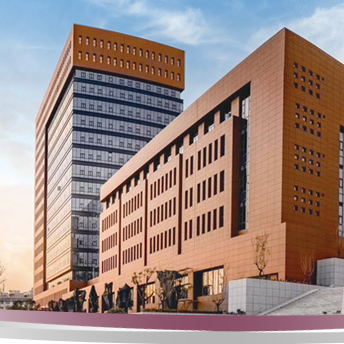
\includegraphics[width=0.3\linewidth]{hutb_building.png}
    \caption{插图示例}
    \label{f.example}
\end{figure}


如果一个图由多个分图(子图)组成,应通过(a),(b),(c)进行标识并附注在分图(子图下方)。
目前子图标识不居中问题没有解决,预计下个版本修复。

\subsection{横向布局}

模板提供常见的图片布局,比如单图布局\ref{f.example},另外还有横排布局如下:

\begin{figure}[!htb]
    \centering
    \begin{subfigure}[t]{0.24\linewidth}
        \begin{minipage}[b]{1\linewidth}
        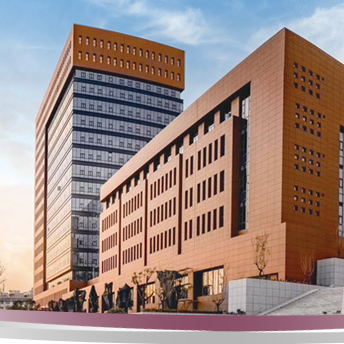
\includegraphics[width=1\linewidth]{hutb_building.png}
        \caption{test}
        \end{minipage}
    \end{subfigure}
    \begin{subfigure}[t]{0.24\linewidth}
        \begin{minipage}[b]{1\linewidth}
        \includegraphics[width=1\linewidth]{hutb_eim.png}
        \caption{test}
        \end{minipage}
    \end{subfigure}
    \begin{subfigure}[t]{0.24\linewidth}
        \begin{minipage}[b]{1\linewidth}
        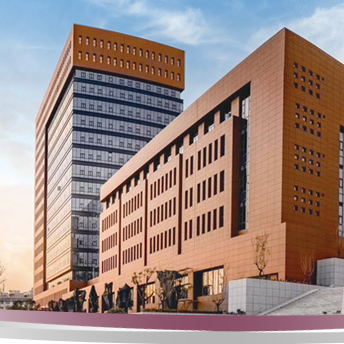
\includegraphics[width=1\linewidth]{hutb_building.png}
        \caption{test}
        \end{minipage}
    \end{subfigure}
    \begin{subfigure}[t]{0.24\linewidth}
        \begin{minipage}[b]{1\linewidth}
        \includegraphics[width=1\linewidth]{hutb_eim.png}
        \caption{test}
        \end{minipage}
    \end{subfigure}
    \caption{图片横排布局示例}
    \label{f.row}
\end{figure}

\section{纵向布局}

纵向布局如图\ref{f.col}

\begin{figure}[!htb]
    \centering
    \begin{subfigure}[t]{0.15\linewidth}
        \captionsetup{justification=centering} %ugly hacks
        \begin{minipage}[b]{1\linewidth}
        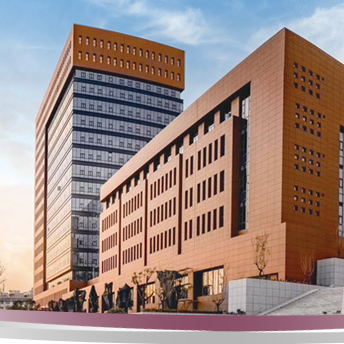
\includegraphics[width=1\linewidth]{hutb_building.png}
        \caption{test}
        \end{minipage}
    \end{subfigure}\\
    \begin{subfigure}[t]{0.15\linewidth}
        \captionsetup{justification=centering} %ugly hacks
        \begin{minipage}[b]{1\linewidth}
        \includegraphics[width=1\linewidth]{hutb_eim.png}
        \caption{test}
        \end{minipage}
    \end{subfigure}
    \caption{图片纵向布局示例}
    \label{f.col}
\end{figure}

\section{竖排多图横排布局}

\begin{figure}[!htb]
    \centering
    \begin{subfigure}[t]{0.13\linewidth}
        \captionsetup{justification=centering} 
        \begin{minipage}[b]{1\linewidth}
        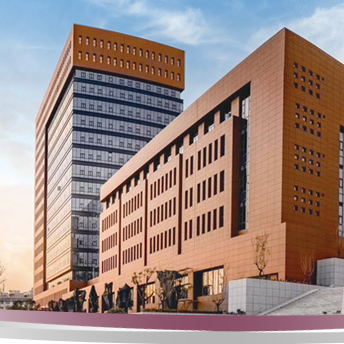
\includegraphics[width=1\linewidth]{hutb_building.png} 
        \vspace{-1ex} \vfill
        \includegraphics[width=1\linewidth]{hutb_eim.png}
        \caption{aaa}
        \end{minipage}
    \end{subfigure}
    \begin{subfigure}[t]{0.13\linewidth}
        \captionsetup{justification=centering} 
        \begin{minipage}[b]{1\linewidth}
        \includegraphics[width=1\linewidth]{hutb_eim.png} 
        \vspace{-1ex} \vfill
        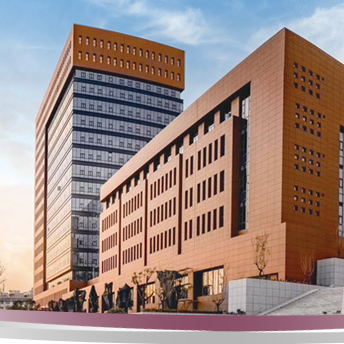
\includegraphics[width=1\linewidth]{hutb_building.png}
        \caption{bbb}
        \end{minipage}
    \end{subfigure}
    \caption{图片竖排多图横排布局}
    \label{f.csu_col_row}
\end{figure}

竖排多图横排布局如图\ref{f.csu_col_row}所示。注意看(a)、(b)编号与图关系


\section{横排多图竖排布局}

潮涌湘江阔,鹏翔天地宽。湖南工商大学正以习近平新时代中国特色社会主义思想为指引,秉持“新工科+新商科+新文科”与理科融合发展的思路,努力形成一流的理念、一流的目标、一流的标准、一流的质量、一流的机制,打造创新工商、人文工商、艺术工商、体育工商、数智工商、绿色工商、幸福工商,建设读书求知的好园地,乘高等教育改革奋进的东风,朝着创新型一流工商大学的愿景扬帆远航。

\begin{figure}[!htb]
    \centering
    \begin{subfigure}[t]{0.3\linewidth}
        \captionsetup{justification=centering} 
        \begin{minipage}[b]{1\linewidth}
        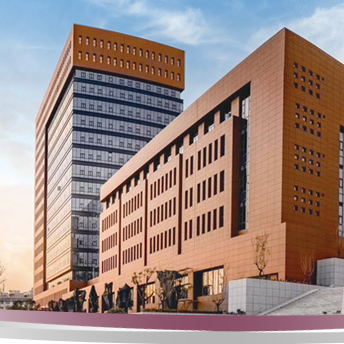
\includegraphics[width=0.45\linewidth]{hutb_building.png}
        \includegraphics[width=0.45\linewidth]{hutb_eim.png}
        \caption{}
        \end{minipage}
    \end{subfigure}\\
    \begin{subfigure}[t]{0.3\linewidth}
        \captionsetup{justification=centering} 
        \begin{minipage}[b]{1\linewidth}
        \includegraphics[width=0.45\linewidth]{hutb_eim.png}
        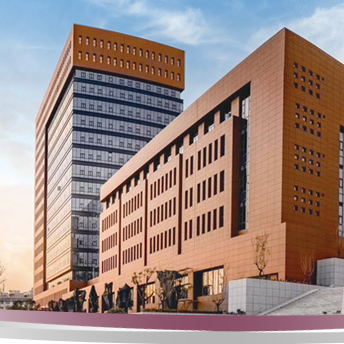
\includegraphics[width=0.45\linewidth]{hutb_building.png}
        \caption{}
        \end{minipage}
    \end{subfigure}
    \caption{图片横排多图竖排布局}
    \label{f.csu_row_col}
\end{figure}

横排多图竖排布局如图\ref{f.csu_row_col}所示。注意看(a)、(b)编号与图关系。

\newpage